\title{CS 180 Homework 2}
\date{\today}

\documentclass[12pt]{article}
\usepackage[margin=1in]{geometry}
\usepackage{enumerate}
\usepackage{scrextend}
\usepackage{filecontents,tikz}
\usepackage{pgfplots}
\usepackage{listings}
\usepackage{graphicx}
\usepackage{svg}
\pgfplotsset{compat=1.7}

\begin{document}
\maketitle

\section{Scheduling}\label{scheduling}
\begin{addmargin}[2em]{2em}
The problem can be approached with greed, by at each point picking the job that maximizes the ratio of weight to completion time. This algorithm looks as follows:
\begin{lstlisting}
Let W be an array of weights of size n
Let T be an array of completion times of size n
Let R be an empty map of size n
For i = 0 to n-1
    Set ratio to W[i] / T[i]
    Append (i, ratio) to R
Sort R from high to low by the values (ratios)
Let W1 be an empty array of size n
Let T1 be an empty array of size n
For i = 0 to n-1
    Append W[R.getkey(i)] to W1
    Append T[R.getkey(i)] to T1
Return W1 and T1
\end{lstlisting}
\end{addmargin}

\section{Degree Sequences}\label{degree sequences}
\begin{enumerate}[(a)]
\item Give a polynomial-time algorithm (in pseudocode) that determines, for a given degree sequence — a
list of node degree values $d_1 \geq d_2 \geq ... \geq d_n \geq 0$ — whether there is an undirected graph $G = (V,E)$ that has these degrees.
\begin{addmargin}[2em]{2em}
\begin{lstlisting}
Let S to be the array of node degrees
For degree in S
    Add degree to sum
If sum is odd
    Return false
Set U to be a an empty array
For degree in S
    If degree is odd
        Push degree to U
        Remove degree from S
If U length is even
    Return true
Otherwise
    Return false
\end{lstlisting}
\end{addmargin}
\item Determine the specific complexity of your algorithm.
\begin{addmargin}[2em]{2em}
The algorithm first loops through $S$, giving $O(n)$ complexity. It then determinse if the sum is odd, which is $O(1)$ complexity. Then it loops through $S$ again, which is again $O(n)$ complexity. As a result, the complete algorithm is $O(n)$.
\end{addmargin}
\item Using your algorithm, determine whether there is a graph with node degrees [5 4 3 2 2 2 2].
\begin{addmargin}[2em]{2em}
First we determine that the sum of the degrees is 20, which is even, so it passes the first test. We then initialize U to be the set of odd degrees, being [3 5]. As the length of U is even, we can safely return true. Therefore there is a graph with this sequence of degrees.
\end{addmargin}
\item Can two non-isomorphic (topologically different) graphs have the same degree sequence?
\begin{addmargin}[2em]{2em}
Graphs that are isomorphic will have the same degree sequence, but the converse is not true. Meaning that non-isomorphic graphs can also have the same degree sequence. The algorithm that I have designed showcases this ambiguity. In showing that the size of U is even, nodes with odd degrees are paired off, but the way in which these nodes are paired is ambiguous, giving multiple possible forms of graphs.
\end{addmargin}
\end{enumerate}

\section{Clique}\label{clique}
\begin{addmargin}[2em]{2em}
\begin{lstlisting}
Let S be a set of all nodes in G
Let H be an empty graph
Let r be some node in G
Remove r from S
Append r to H
Let Size be equal to 1
For node in S
    If BlackBox(H + node, Size + 1) is true
        Remove node from S
        Append node to H
Return Size
\end{lstlisting}
The time complexity of the algorithm is clearly $O(n)$, simply due to the for loop, which at the worst case loops through every node in graph $G$. All other operations are $O(1)$ complexity.
\end{addmargin}

\section{Shortest Paths}\label{shortest paths}
\begin{enumerate}[(a)]
\item Please explain how the proof of (4.14) on p.139 fails if edge lengths can be negative.
\begin{addmargin}[2em]{2em}
The proof (4.14) in the [KT] text shows that Dijkstra's algorithm holds true fora ll graphs containing entirely positive edge lengths. However, the proof potentially fails with the existence of negative edge lengths. Specifically, it fails because of the following statement: "$P$ cannot be shorter than $P_v$ because it is already at least as long as $P_v$". This is, however, not true with negative lengths, as the addition of a negative edge length to $P_v$ will inevitably reduce the length of $P$, causing the induction proof to fail in the $k + 1$ instance.
\end{addmargin}
\item With these distances, the shortest-path distances between LAX and other major airports in the US (in miles), and print the shortest-path tree of all shortest paths from LAX, with distances. If you prefer, you can plot the shortest path tree, using (longitude,latitude) as (x,y) positions.\\
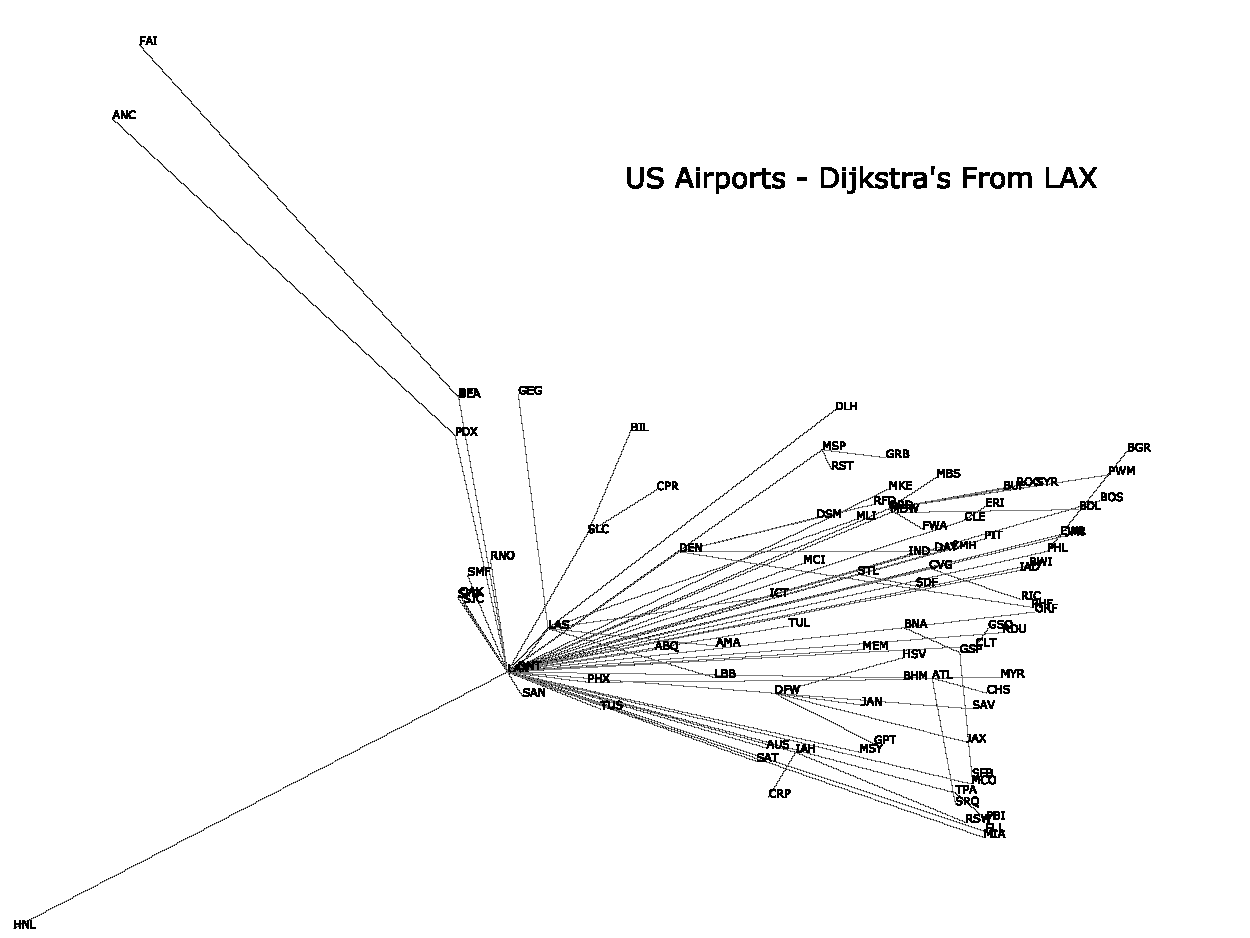
\includegraphics[width=\textwidth]{dijkstras-lax}
\end{enumerate}

\section{Minimum Spanning Tree}\label{minimum spanning tree}
\begin{enumerate}[(a)]
\item Prove or disprove: if all the edge weights in a graph are distinct, then the MST is unique.
\begin{addmargin}[2em]{2em}
We can prove this by contradiction. We assume that there are two different minimum spanning trees $T_1$ and $T_2$ and assume there exists an edge with lowest cost $e_1$ in $T_1$ but not in $T_2$. By definition of a MST, $T_2$ with the edge $e_1$ wil contain some cycle. This cycle will then contain an edge $e_2$, which has greater cost than $e_1$, by the definition of the assumption. Therefore, the cycle must contain one edge that is not in $T_1$ to avoid contradiction with the definition of being an MST. Finally, replacing $e_2$ with $e_1$ results in a spanning tree with less overall cost. Which means that the original tree $T_2$ was not a spanning tree, which is a contradiction.
\end{addmargin}
\item Prove or disprove: in an undirected graph $G$, there can be a central node $s$ for which the shortest path tree from $s$ has lower total edge length than the minimum spanning tree.
\begin{addmargin}[2em]{2em}
Given that the shortest path tree from $s$, must contain all point in $G$, it is possible to disprove the notion of the shortest path tree have lower total edge length than the MST simply by proving the correctness of a MST algorithm in achieving a tree with minimum total cost. This can be done simply using proof (4.19) from the [KT] text.
\end{addmargin}
\item Using the distance values you derived in the previous problem, compute the Minimum Spanning Tree (MST) for the US airport network. Determine whether all the edge weights (distances, here) are distinct (however: all distance matrix values are integers). Extract the path from Los Angeles (LAX) to Washington DC (IAD) through the MST. Compare this path with the shortest path to IAD in the shortest-path tree from LAX.
\begin{addmargin}[2em]{2em}
The MST below was created using a python script that I wrote which utilizes a variation on Prim's algorithm to create the minimum spanning tree. The shortest path from LAX to IAD on this tree is LAX-LAS-PHX-TUS-ABQ-DEN-AMA-DFW-AUS-IAH-MSW-BHM-ATL-GSP-CLD-RDU-IAD, while in the shortest-path tree, the path is simply LAX-IAD. Furthermore, all edges are of distinct, unique length.
\end{addmargin}
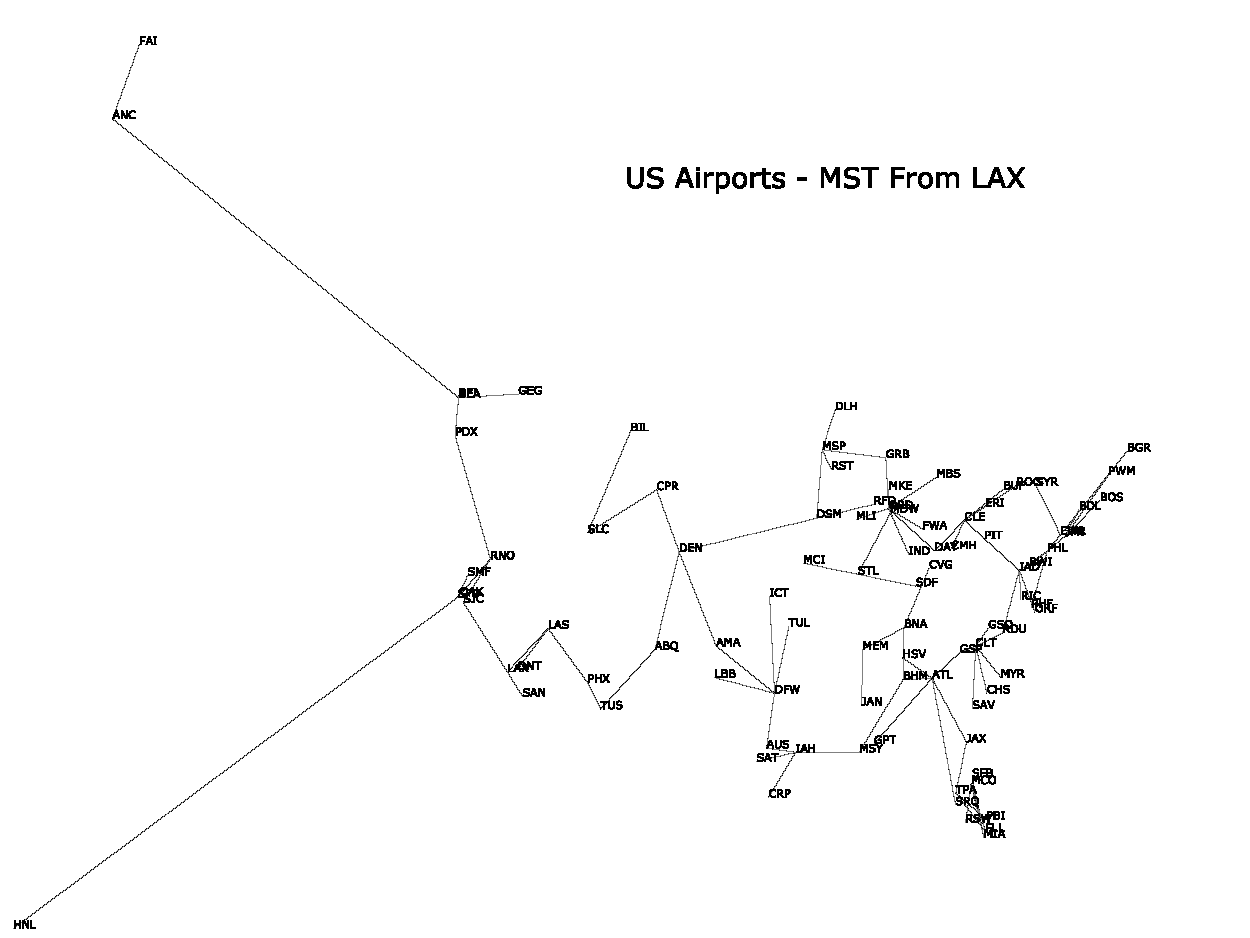
\includegraphics[width=\textwidth]{mst-lax}
\item Using the Maximal Separation Clustering approach described in section 4.7 of the text, find a clustering of the airports into four clusters using the MST. Specify the airports in each cluster. (Hint: this can be done visually.)
\begin{addmargin}[2em]{2em}
We can create the clustering into four clusters simply by removing the largest edges. The edges removed are ANC-SEA, HNL-SFO, DEN-RFD. The result is shown below:
\end{addmargin}
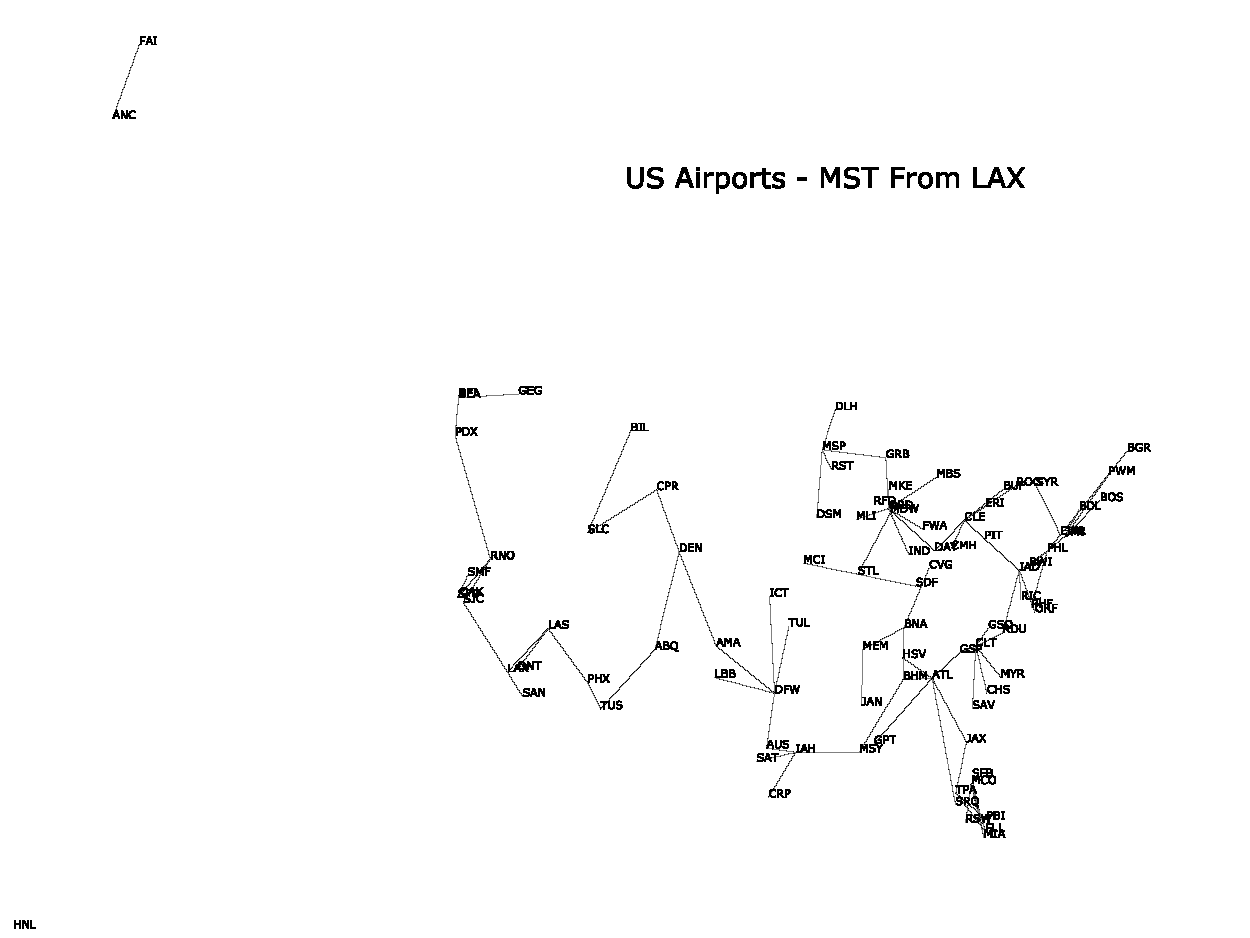
\includegraphics[width=\textwidth]{cluster-lax}
\item A congestion spanning tree of an undirected graph $G$ is a spanning tree in which the largest edge weight is minimum over all spanning tree of $G$. The value of the congestion spanning tree is the weight of its maximum-weight edge.
\begin{enumerate}[i.]
\item Argue that the every MST is also a congestion spanning tree.
\begin{addmargin}[4em]{2em}
A spanning tree is the minimum when its sum of edge weights is the minimum over all spanning trees of graph $G$. It follows that if a single edge weight is minimum over all spanning trees, and that the sum of edge weights is greater than any single edge weight, then every minimum spanning tree is also a congestion spanning tree.
\end{addmargin}
\item Given a linear-time algorithm that, given a graph $G$ and an integer $b$, determines whether the value of the congestion spanning tree is at most $b$. In other words, determine whether the maximum edge cost $c$ of the congestion spanning tree satisfies $c \leq b$.
\begin{addmargin}[4em]{2em}
Given that it can be determined if a graph $G$ has a congestion spanning tree of at most value $b$, and that the value of a congestion tree is equal it its most expensive edge, it is fairly clear the cost of the the maximum-cost edge $c$ is upper-bounded by $b$, simply by the definition of a congestion spanning tree. Therefore, the condition, $c \leq b$, is satisfied.
\end{addmargin}
\end{enumerate}
\end{enumerate}
\end{document}